
\section{Doping determination}
    \label{Sec:ResH:DopingDetermination}

As described in section~\ref{Sec:Intro:DeterminingDoping}, we compared the Hall values of our samples at high temperature to determine the doping similar to the method used by Ando \etal\cite{Ando2000}. In order to compare this method with other doping characterisation methods, the actual (i.e. not nominal) $T_c$ values for the samples were used from the resistivity curves shown in figure~\ref{Fig:ResH:TSweeps}. These values were input into the parabolic relation from Presland \etal~\cite{Presland1991} and Ando \etal~\cite{Ando2000}. This is then compared with the doping assignments which we make by matching $R_H(\unit{300}{\kelvin})$ in the \ac{BSCO} data from the previous section with that compiled in Kokalj \etal~\cite{Kokalj2012} on \ac{TL2201}. The results of these comparisons are shown in figure~\ref{Fig:ResH:DopingRh300}.
\begin{figure}[htbp]
    \begin{center}
        \includegraphics[scale=0.9]{Chapter-HallBSCO/Figures/DopingRh300/DopingRh300}
        \caption{Assigning the dopings of the \ac{BSCO} data such that $R_H(\unit{300}{\kelvin})$ values match those of \ac{TL2201}. Dashed line is a second order polynomial fit to the \ac{TL2201} data that is used to obatin the exact dopings.}
        \label{Fig:ResH:DopingRh300}
    \end{center}
\end{figure}
The \ac{TL2201} data does not span the entire range of $R_H(\unit{300}{\kelvin})$ values that the \ac{BSCO} covers, for this reason a second order polynomial is fit to the Kokalj data and the \ac{BSCO} doping is assigned to this curve. The underdoped sample B28KUD3a is far along the extrapolated curve, however still lies within the standard Presland/Tallon assignment as used to determine the dopings for the Konstantanovic data~\cite{Konstantinovic2001}.

Figure~\ref{Fig:ResH:Dopings} shows the dopings as determined by the three different methods outlined in the experimental methods chapter. The dopings of the crystals range from $p=0.12$ to $p=0.36$ hole per Cu atom with significant discrepancies between the methods. The Ando determination bunches the doping values around a much narrower range, whereas the dopings determined by comparing with the \ac{TL2201} \ac{dHvA} data, spread the overdoped values over a wider range. The Presland/Tallon method sits between the two. Most notable is that the dopings assigned by Kondo \etal~\cite{Kondo2004} from \ac{ARPES} measurements of the Fermi surface volume. These are for different samples from the same growth batch but show significantly higher still span of dopings between $p=0.25$ and $p=0.43$. It is not clear why there is a discrepancy, however a possible explanation for the larger doping values from the \ac{ARPES} measurements is that \ac{ARPES} is susceptible  to surface charging effects which could influence the apparent size of the Fermi surface volume at the cleaved physical surface.

\begin{figure}[htbp]
    \begin{center}
        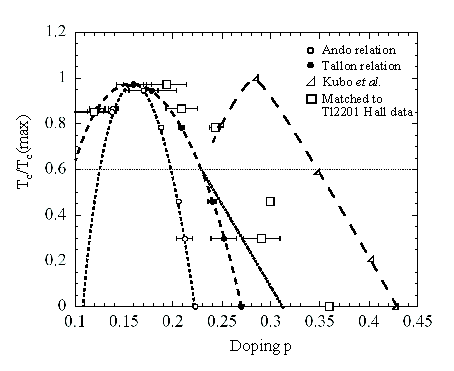
\includegraphics[scale=1.1]{Chapter-HallBSCO/Figures/Dopings/Dopings}
        \caption{Doping distributions for the three different methods. From left to right, B28KUD3A, B30KUD3 (Assume UD), B32KOP1, B32KOP4, B30KUD3 (Assume OD), B30KOD3, B16KOD1A, B07KOD2, B00KOD1A. Broken lines are a guide to the eye. Circled points are B30KUD3 for both the overdoped and underdoped scenarios.}
        \label{Fig:ResH:Dopings}
    \end{center}
\end{figure}

% \begin{figure}[htbp]
%     \begin{center}
%         \includegraphics[scale=1.2]{Chapter-HallBSCO/Figures/DRhoDtCurves/DRhoDtCurves}
%         \caption{$d\rho(T)/dT$ curves for each of the samples taken in \unit{0}{\tesla} and \unit{13}{\tesla} field. Note the evolution of the $T_{\textrm{coh}}$ gradient in the overdoped samples which give way to the $T^*$ kink in the underdoped samples, B30KUD3 has been repositioned to follow this trend.}
%         \label{Fig:ResH:DRhoDtCurves}
%     \end{center}
% \end{figure}
% The derivatives of the same resistivity curves in figure~\ref{Fig:ResH:TSweeps} are plotted in figure~\ref{Fig:ResH:DRhoDtCurves} along with derivatives to temperature sweeps taken at \unit{13}{\tesla}. Here we can see in the overdoped samples the distinct slope downwards towards \Tc which signifies the coherent quasiparticle region which begins at $T_{\textrm{coh}}$. This gradually levels out as doping is reduced until we observe a kink which marks the pseudogap temperature, $T^*$. The $T^*$ kink is weaker in B30KUD3 than the optimally doped samples and in fact only appears, at a much lower temperature, when the field is applied. This suggests that it is in fact more doped than the optimally doped samples rather than less doped as the nominal composition would suggest. If we consider B30KUD3 to be overdoped rather than underdoped then this trend continues right across the range of samples.


% Figure~\ref{Fig:ResH:Rh300Comparison} present Hall data at \unit{300}{\kelvin} again taken in the Polo with comparable data from Konstantinovi\'c \etal~\cite{Konstantinovic2001}.
% \begin{figure}[htbp]
%     \begin{center}
%         \includegraphics[scale=1.1]{Chapter-HallBSCO/Figures/Rh300Comparison/Rh300Comparison}
%         \caption{Hall data at \unit{300}{\kelvin} compared with similar data taken from refs.~\cite{Konstantinovic2001, Kokalj2012} using different doping assignments. From left: Tallon relation, Ando relation and scaling to \ac{TL2201} data. Red lines are guides to the eye, circled points are B30KUD3 in the overdoped and underdoped positions.}
%         \label{Fig:ResH:Rh300Comparison}
%     \end{center}
% \end{figure}
% It is clear that the Ando assignment of dopings is too confined with the data not at all following the respective curves whereas the Tallon relation follows much close the shape of the curve, although, perhaps this is not surprising given that the dopings in the Konstantinovo\'c paper were also assigned using the Tallon relation. However what is most interesting is that when compared with \ac{TL2201} data from Kokalj \etal~\cite{Kokalj2012} which we know is appropriate to scale to the \ac{TL2201} doping scheme, we see that of the three methods, scaling the \ac{BSCO} to the \ac{TL2201} \ac{dHvA} data matches the closest. On this rationale, we continue assuming that the \ac{TL2201} doping assignments are the correct ones.

% Also, referring to the circled points, we see that again the data is more consistent if we consider the B30KUD3 to be overdoped rather than underdoped. Looking back to the inset of figure~\ref{Fig:ResH:TSweeps} we see that there is large scatter in the data points due to uncertainty in the dimensions which were determined by optical microscope, however there is an approximate downward trend with doping which is similar to what is found in the literature~\cite{Ando2000, Ando1999, Konstantinovic2001, Ono2000}. Although B30KUD3 is more consistent to this trend in the underdoped position, the trend still lies with the error bars of the overdoped position. Looking ahead to the inset of figure~\ref{Fig:ResH:InvHallCombined} which shows $R_H$ values at \unit{300}{\kelvin} vs. doping, which depend only on the measurement of depth --- which was much more accurately determined by the \ac{FIB} --- we see that the underdoped position lies far outside the overall trend even when considering the error bars. 

